\documentclass[12pt]{article}
\renewcommand{\labelenumii}{\theenumii}
\renewcommand{\theenumii}{\theenumi.\arabic{enumii}.}
\usepackage[utf8]{inputenc}
%\usepackage[T1]{fontenc}

\usepackage{geometry}
\geometry{a4paper}
\usepackage{graphicx}
\usepackage{float}
\usepackage[italian]{babel}

\linespread{1.2}
\setlength{\parindent}{0pt}

\begin{document}

%----------------------------------------------------------------------------------------
%	TITOLO
%----------------------------------------------------------------------------------------

\begin{titlepage}

\newcommand{\HRule}{\rule{\linewidth}{0.5mm}}

\center

\textsc{\Large Relazione di progetto di "Smart City e Tecnologie Mobili"}\\[0.5cm]

\HRule \\[0.4cm]
{ \huge \bfseries Smart Public Restroom }\\[0.4cm]
\HRule \\[1.5cm]

\vfill

\begin{flushleft}
\emph{Numero del gruppo:}\\[1cm]
\emph{Componenti del gruppo:}\\[3cm]
\end{flushleft}



\end{titlepage}

%----------------------------------------------------------------------------------------
%	INDICE
%----------------------------------------------------------------------------------------

\tableofcontents

\newpage

%----------------------------------------------------------------------------------------
%	INTRODUZIONE
%----------------------------------------------------------------------------------------

\section{Introduzione}

Esporre l’obiettivo del progetto dandone una visione complessiva.\\

Devono essere illustrate le caratteristiche salienti del progetto; deve essere chiara la distinzione tra le tecnologie usate/assemblate durante lo svolgimento dell'elaborato e il contributo tecnologico/scientifico effettivamente apportato dal gruppo.\\


Vincoli circa la lunghezza della sezione (escluse didascalie, tabelle, testo nelle immagini, schemi):

\vspace{1cm}
\begin{tabular}{l|rr}
 & Numero minimo di battute & Numero massimo di battute \\
 \hline
 1 componente & 2000 & 3000 \\
 2 componenti & 2500 & 4500 \\
 3 componenti & 3000 & 6000 \\
 \hline
\end{tabular}


\newpage


%----------------------------------------------------------------------------------------
%	STATO DELL'ARTE
%----------------------------------------------------------------------------------------

\section{Stato dell'arte}

Riassumere le soluzioni presenti in letteratura inerenti al problema in esame. Per ciascuna, discutere le principali diversità o affinità rispetto al progetto presentato. Nel caso non siano presenti soluzioni direttamente comparabili a quella presentata descrivere comunque le principali tecniche note per affrontare la tematica trattata.\\

Le soluzioni esposte devono essere corredate degli opportuni riferimenti bibliografici. Nel caso si tratti di soluzioni già operative sul mercato, devono essere indicate le fonti (online) dove poter accedere al servizio o approfondirne i contenuti.\\


Vincoli circa la lunghezza della sezione (escluse didascalie, tabelle, testo nelle immagini, schemi):

\vspace{1cm}
\begin{tabular}{l|rr}
 & Numero minimo di battute & Numero massimo di battute \\
 \hline
 1 componente & 2000 & 3000 \\
 2 componenti & 2500 & 4500 \\
 3 componenti & 3000 & 6000 \\
 \hline
\end{tabular}


\newpage


%----------------------------------------------------------------------------------------
%	ANALISI DEI REQUISITI
%----------------------------------------------------------------------------------------

\section{Analisi dei requisiti}

In questa sezione esporre brevemente i requisiti a cui il sistema proposto deve rispondere, concentrando l'attenzione sugli aspetti più rilevanti e facendo eventualmente uso di opportuni diagrammi di alto livello.\\

Vincoli circa la lunghezza della sezione (escluse didascalie, tabelle, testo nelle immagini, schemi):

\vspace{1cm}
\begin{tabular}{l|rr}
 & Numero minimo di battute & Numero massimo di battute \\
 \hline
 1 componente & 4000 & 6000 \\
 2 componenti & 6000 & 8000 \\
 3 componenti & 8000 & 10000 \\
 \hline
\end{tabular}


\newpage

\subsection{Requisiti}

È necessario realizzare un sistema di gestione per bagni pubblici che consenta a un utente amministrativo, da remoto, di visionare lo stato generale di un impianto.\\
Nel dettaglio ci si aspetta che un utente possa, dato uno specifico impianto, visualizzare in tempo reale:
\begin{itemize}
\item Indicazioni sulla quantità di sapone per le mani rimasto in ogni dispenser, indicato in centesimi.
\item Indicazioni sul tasso di riempimento di ogni pattumiera presente, indicata in centesimi.
\item Indicazioni sullo stato aperto/chiuso di ogni singola cella dell'impianto.
\item Indicazioni sullo stato disponibile/terminata di ogni dispenser di carta igienica presente nelle celle dell'impianto.
\item Indicazioni sullo stato funzionante/non funzionante delle luci di cortesia ad ogni cella.
\item Indicazioni sul tasso di umidità di ogni cella dell'impianto.
\end{itemize}
Le informazioni sopra riportate dovranno essere visionabili attraverso un apposita web app chiamata \textit{manager}, che fungerà da supporto gestionale dei bagni pubblii installati.\\
A fronte infatti di un semplice autenticazione tramite utente/password, infatti, l'app dovrà inoltre consentire di: 
\begin{itemize}
\item Aggiungere nuovi impianti al sistema.
\item Visualizzare e, all'occorrenza, modificare alcune informazioni di carattere generale sui bagni pubblici installati, come ad esempio indirizzo, coordinate GPS e azienda di manutenzione assegnata.
\item Aggiungere nuovi utenti di amministrazione.
\item Visualizzare eventuali report utente sullo stato del sistema dell'app \textit{consumer}.
\end{itemize}
Si dovrà anche fornire un apposita app web (chiamata \textit{consumer}) a supporto di tutti i cittadini che si vogliono recare in un ambito pubblico in un certo momento della giornata.\\
L'app, infatti, dovrà mostrare a schermo la locazione di ogni bagno pubblico disponibile e, all'occorrenza, riportare lo stato degli stessi: qualora un bagno pubblico non sia agibile per qualche motivo, tale informazione dovrà essere opportunamente riportata.\\
Nel dettaglio, l'app \textit{consumer} dovrà consentire di:
\begin{itemize}
\item Visualizzare una \textit{gmap} (centrata sulla locazione corrente) con indicati i bagni pubblici disponibili del sistema.\\Ogni bagno, se selezionato, dovrà mostrare informazioni utili al cittadino circa il loro stato corrente.
\item Riportare direttamente dall'app di eventuali problemi dell'applicazione/dei bagni pubblici riscontrati.
\end{itemize}
\newpage
\subsection{Analisi dei requisiti}
\subsubsection{Glossario}

\begin{center}
    \begin{tabular}{ | l |  p{10cm} |}
    \hline
    \textbf{Name} & \textbf{Definition} \\ \hline
    Impianto & Struttura rappresentante un bagno pubblico, contenente una serie di celle individuali. Ogni impianto è comprensivo di lavabi, dispenser di sapone e pattumiere. \\ \hline
    Cella & Struttura rappresentante una singola unità per servizi igienici comprensiva di gabinetto, carta igienica e luce di cortesia. \\ \hline
    `Manager` web App & Applicazione di amministrazione impianti utilizzata per gestire l'insieme dei bagni pubblici registrati nel network.\\ \hline
    `Consumer` web App & App di supporto al cittadino per individuare il più vicino bagno pubblico e visionare il suo stato corrente.\\ \hline
    gmap & Mappa geolocalizzata 2D fornita gratuitamente da \textit{Google} e molto conosciuta tra gli utenti.\\ \hline
    Utente amministrativo & Utente adibito a compiti di amministrazione e gestione dei bagni pubblici registrati nella rete, attraverso la web app \textit{manager}.\\ \hline
    Utente consumer & Utente della web app \textit{consumer}. \\ \hline
    \end{tabular}
\end{center}	
\newpage
\subsubsection{Casi d'uso}

\begin{figure}[h!]
  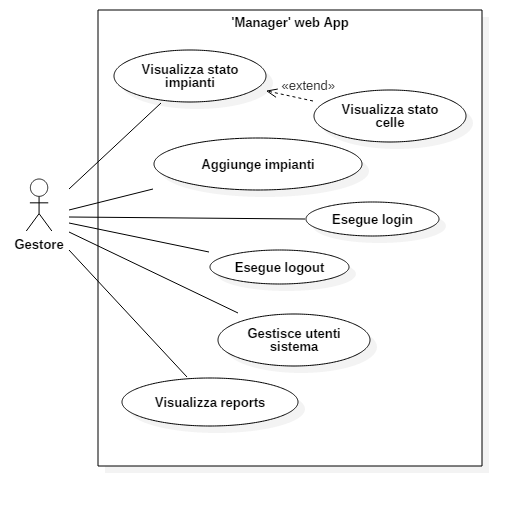
\includegraphics[scale=0.7]{img/usecase_manager.png}
  \caption{Casi d'uso per l'app `manager`}
  \label{fig:usecase_manager}
\end{figure}
\begin{figure}[h!]
  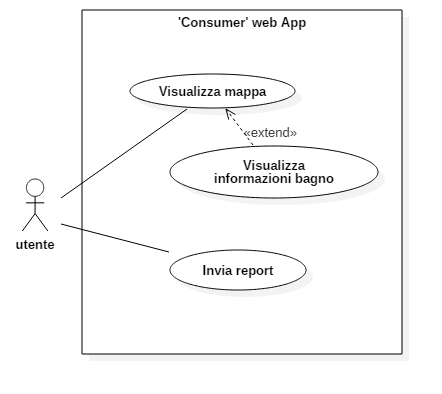
\includegraphics[scale=0.7]{img/usecase_consumer.png}
  \caption{Casi d'uso per l'app `consumer`}
  \label{fig:usecase_consumer}
\end{figure}
\newpage
\phantom{}
\newpage
\subsubsection{Requisiti funzionali}
\begin{enumerate}

\item L'app \textit{manager} richiederà obbligatoriamente un'autenticazione nella forma login/password.
\item Gli utenti di \textit{manager} dovranno essere in grado di visualizzare i dati inviati dai sensori in tempo reale.
\item Ogni impianto dovrà rendere disponibili i seguenti dati:
\begin{itemize}
\item Sapone residuo di ogni dispenser, espresso in centesimi.
\item Spazio residuo (tasso di riempimento) di ogni pattumiera, espresso in centesimi.
\end{itemize}
Per ogni cella, inoltre, saranno richiesti i seguenti dati:
\begin{itemize}
\item Segnalazione esaurimento carta igienica.
\item Stato di apertura della porta di accesso.
\item Tasso di umidità.
\item Ssegnalazione guasto della luce di cortesia.
\end{itemize}
\end{enumerate}
\subsubsection{Requisiti non funzionali}
%----------------------------------------------------------------------------------------
%	PROGETTAZIONE
%----------------------------------------------------------------------------------------

\section{Progettazione}

Devono essere esposte le scelte progettuali operate nelle varie fasi di sviluppo dell'elaborato.\\

In questa sezione devono essere documentati gli schemi di progetto relativamente all'architettura complessiva del sistema e alle sue componenti di rilievo che possano meritare un'analisi di dettaglio. Per le componenti software si può ricorrere ad esempio a diagrammi delle classi, di sequenza, stato, attività. Per le componenti hardware è possibile includere opportuni schemi in grado di descrivere l'architettura fisica adottata.\\

Vincoli circa la lunghezza della sezione (escluse didascalie, tabelle, testo nelle immagini, schemi):

\vspace{1cm}
\begin{tabular}{l|rr}
 & Numero minimo di battute & Numero massimo di battute \\
 \hline
 1 componente & 9000 & 18000 \\
 2 componenti & 12000 & 21000 \\
 3 componenti & 15000 & 24000 \\
 \hline
\end{tabular}


\newpage


%----------------------------------------------------------------------------------------
%	IMPLEMENTAZIONE
%----------------------------------------------------------------------------------------

\section{Implementazione}\label{sec:implementazione}

Esporre i principali problemi affrontati durante l'effettiva realizzazione delle componenti hardware/software e illustrare le soluzioni implementative adottate. Se l'elaborato ha previsto l'utilizzo di tecnologie già disponibili sul mercato, discuterne brevemente le caratteristiche e motivarne l'adozione rispetto ad altre soluzioni assimilabili.\\

\textbf{NOTA: in questa sezione devono essere riportate esclusivamente le porzioni di codice ritenute particolarmente significative. Il codice sorgente nella sua interezza, opportunamente commentato, deve essere consegnato separatamente dalla relazione in un archivio compresso.}\\


Vincoli circa la lunghezza della sezione (escluse didascalie, tabelle, testo nelle immagini, schemi):

\vspace{1cm}
\begin{tabular}{l|rr}
 & Numero minimo di battute & Numero massimo di battute \\
 \hline
 1 componente & 5000 & 11000 \\
 2 componenti & 8000 & 16000 \\
 3 componenti & 10000 & 21000 \\
 \hline
\end{tabular}


\newpage


%----------------------------------------------------------------------------------------
%	TESTING E PERFORMANCE
%----------------------------------------------------------------------------------------

\section{Testing e performance}

Esporre lo stato di funzionamento effettivo del sistema progettato ad elaborato concluso. Per ciascuna delle funzionalità salienti devono essere tabellate e discusse le performance riscontrate mediante opportuni test eseguiti in fase di validazione del progetto.\\

I tempi di esecuzione/comunicazione devono essere accompagnati dalle caratteristiche dell'hardware sul quale è eseguito il software.\\

Qualora l'elaborato includa algoritmi innovativi, indicarne la complessità computazionale (avendo cura di esporre lo pseudo codice nella sezione \ref{sec:implementazione}).\\


Vincoli circa la lunghezza della sezione (escluse didascalie, tabelle, testo nelle immagini, schemi):

\vspace{1cm}
\begin{tabular}{l|rr}
 & Numero minimo di battute & Numero massimo di battute \\
 \hline
 1 componente & 2000 & 3000 \\
 2 componenti & 2500 & 4500 \\
 3 componenti & 3000 & 6000 \\
 \hline
\end{tabular}


\newpage


%----------------------------------------------------------------------------------------
%	ANALISI DI DEPLOYMENT SU LARGA SCALA
%----------------------------------------------------------------------------------------

\section{Analisi di deployment su larga scala}

In questa sezione va discussa, eventualmente con l'ausilio di opportuni diagrammi (componenti, deployment), l'evoluzione del progetto presentato immaginando che venga adottato su larga scala. I dettagli qui esposti devono quindi astrarre dalle specifiche dell'elaborato qualora l'implementazione sia stata focalizzata su uno scenario isolato.\\

A titolo d’esempio, qualora applicabile, devono essere evidenziate le criticità che si potrebbero incontrare e devono essere proposte soluzioni tipiche in contesti di \textit{cloud architecture} per garantire un'adeguata \textit{resilienza}, in termini di \textit{availability} e \textit{scalability} del sistema.\\


Vincoli circa la lunghezza della sezione (escluse didascalie, tabelle, testo nelle immagini, schemi):

\vspace{1cm}
\begin{tabular}{l|rr}
 & Numero minimo di battute & Numero massimo di battute \\
 \hline
 1 componente & 3000 & 6000 \\
 2 componenti & 4500 & 9000 \\
 3 componenti & 6000 & 12000 \\
 \hline
\end{tabular}


\newpage


%----------------------------------------------------------------------------------------
%	PIANO DI LAVORO
%----------------------------------------------------------------------------------------

\section{Piano di lavoro}

In questa sezione devono essere chiariti i compiti svolti da ciascun candidato nel caso in cui il gruppo abbia più di un componente.\\

Deve essere inoltre esposto il piano di lavoro adottato. A tal fine, per ogni attività svolta durante la preparazione dell'elaborato (ad esempio: studio di una tecnologia, progettazione di un componente, implementazione di un algoritmo ecc…) deve essere chiarita la collocazione temporale e devono essere indicate le risorse impiegate per svolgerla (giorni/uomo). I candidati possono ricorrere a opportuni diagrammi come quello di Gantt.\\


Vincoli circa la lunghezza della sezione (escluse didascalie, tabelle, testo nelle immagini, schemi):

\vspace{1cm}
\begin{tabular}{l|rr}
 & Numero minimo di battute & Numero massimo di battute \\
 \hline
 1 componente & 1000 & 2000 \\
 2 componenti & 1500 & 3000 \\
 3 componenti & 2000 & 4000 \\
 \hline
\end{tabular}

\newpage


%----------------------------------------------------------------------------------------
%	CONCLUSIONI
%----------------------------------------------------------------------------------------

\section{Conclusioni}

Esporre brevemente le considerazioni conclusive sul progetto presentato, indicando anche i possibili sviluppi futuri.\\

Vincoli circa la lunghezza della sezione (escluse didascalie, tabelle, testo nelle immagini, schemi):

\vspace{1cm}
\begin{tabular}{l|rr}
 & Numero minimo di battute & Numero massimo di battute \\
 \hline
 1 componente & 500 & 1000 \\
 2 componenti & 1000 & 2000 \\
 3 componenti & 1500 & 3000 \\
 \hline
\end{tabular}

\newpage


%----------------------------------------------------------------------------------------
%	APPENDICE
%----------------------------------------------------------------------------------------

\appendix
\addcontentsline{toc}{section}{Appendice}
\section*{Appendice}
Laddove necessario è possibile avvalersi di appendici alla relazione per includere materiale di approfondimento.\\

A titolo esemplificativo possono essere incluse le schede tecniche dei componenti adottati, la normativa di riferimento che regola un particolare dominio applicativo, ecc.


\newpage


%----------------------------------------------------------------------------------------
%	RIFERIMENTI BIBLIOGRAFICI
%----------------------------------------------------------------------------------------
\addcontentsline{toc}{section}{Riferimenti bibliografici}
\begin{thebibliography}
EElencare i riferimenti bibliografici citati nel testo. 
\end{thebibliography}

%----------------------------------------------------------------------------------------

\end{document}